\section{Calcul d'erreurs}
\label{sec:erreurs}

Les erreurs sur les mesures sont données dans le \autoref{tab:erreurs}.

\begin{table}[h]
    \centering
    \begin{tabulary}{\textwidth}{C C}
        \toprule
        Variable & Erreur \\
        \midrule
        Longueur, largeur, et épaisseur \(L, \ell, e\) [\si{\milli\meter}] & 0.01 \\
        \(U_F\) [\si{\volt}] & 0.001 \\
        \(U_{\Delta L}\) [\si{\volt}] & 0.001 \\
        \bottomrule
    \end{tabulary}
    \caption{Erreurs estimées sur les mesures}
    \label{tab:erreurs}
\end{table}

\paragraph*{Regression linéaire}
Les erreurs sur les régressions linéaires \(y = ax + b\) sur les mesures \((x_i, y_i) ; i = \{1, \dots, n\}\) sont donnés par \cite{erreursmesure}:

\begin{equation}
    \label{eq:erreur:fit}
    \begin{aligned}
        (\Delta a)^2 &= \frac{\sum_{i=1}^{n}(y_i - (a x_i + b))^2}{(n-2) \sum_{i=1}^{n}(x_i - \bar{x})^2}\\
        \Delta b &= \bar{x} \Delta a + a \Delta \bar{x}
    \end{aligned}
\end{equation}

En pratique, ces valeurs sont calculées par la bibliothèque python \texttt{numpy}.

\paragraph*{Formules d'erreurs}

Erreur sur la contrainte de cisaillement \(\sigma\):
\begin{equation}
    \Delta \sigma = \absfrac{\Delta U_F}{U_F} \sigma + \absfrac{\Delta S_0}{S_0} \sigma
\end{equation}
où \(S_0 = \ell e\) est la surface de coupe de l'échantillon avant traction et \(U_F\) est la tension de sortie du capteur de force.

Erreur sur la déformation de cisaillement \(\varepsilon\):
\begin{equation}
    \Delta \varepsilon = \absfrac{\Delta U_{\Delta L}}{U_{\Delta L}} \varepsilon + \absfrac{\Delta L_0}{L_0} \sigma
\end{equation}
où \(L_0\) est la longueur avant traction de l'échantillon et \(U_{\Delta L}\) est la tension de sortie du capteur de déformation.

Toutes ces erreurs sont calculées en pratique par la bibliothèque \texttt{uncertainties}.


% \section{Figures supplémentaires}
% \label{sec:fig_supp}

% \begin{figure}
%     \centering
%     \begin{subfigure}{0.48\linewidth}
%         \centering
%         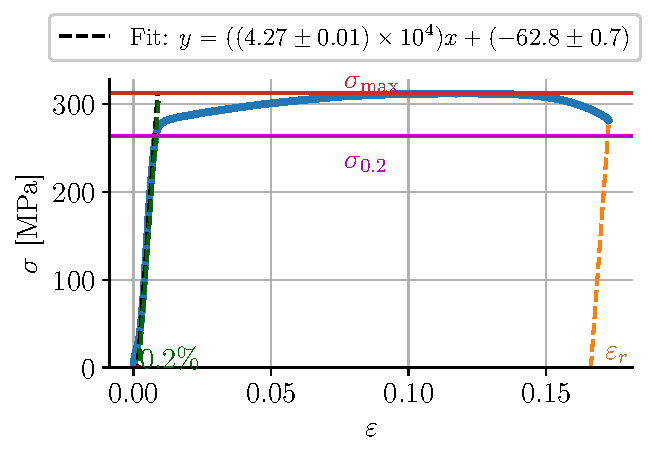
\includegraphics[width=\linewidth]{figures/froid1all.pdf}
%         \caption{}
%         \label{fig:froid1}
%     \end{subfigure}
%     \begin{subfigure}{0.48\linewidth}
%         \centering
%         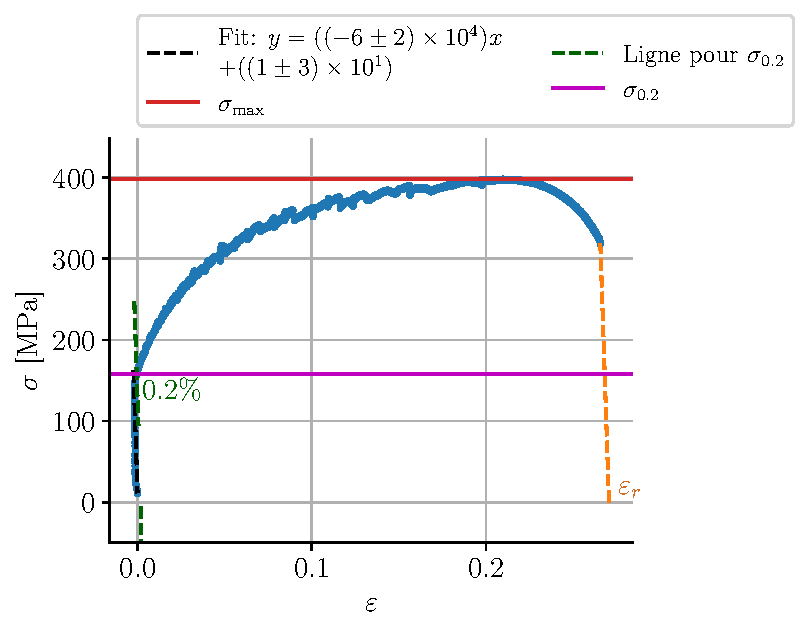
\includegraphics[width=\linewidth]{figures/chaud4all.pdf}
%         \caption{}
%         \label{fig:chaud4}
%     \end{subfigure}
%     \begin{subfigure}{0.48\linewidth}
%         \centering
%         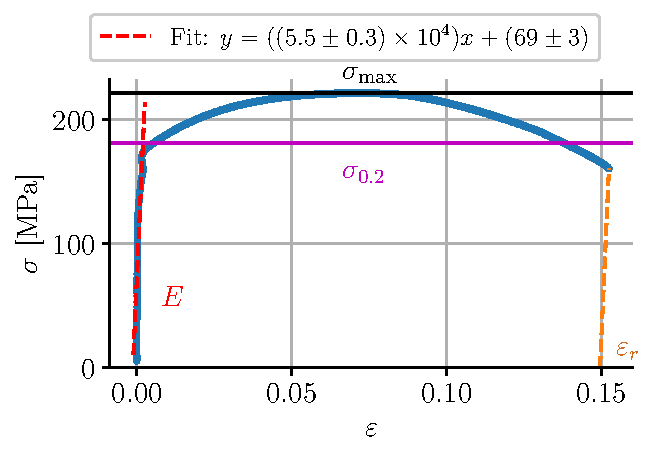
\includegraphics[width=\linewidth]{figures/tiede5all.pdf}
%         \caption{}
%         \label{fig:tiede5}
%     \end{subfigure}
%     \begin{subfigure}{0.48\linewidth}
%         \centering
%         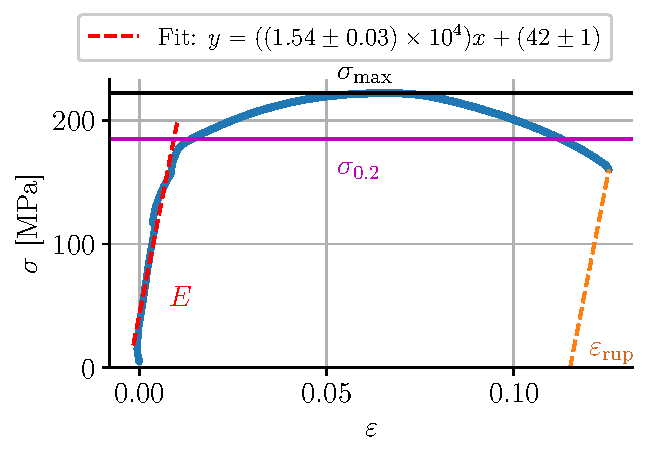
\includegraphics[width=\linewidth]{figures/tiede7all.pdf}
%         \caption{}
%         \label{fig:tiede7}
%     \end{subfigure}
%     \caption{Courbe de traction pour 4 échantillons (a) non-traité (b) adouci (c) et (d) adouci puis durci. Une régression linéaire a été réalisée afin d'obtenir le module de Young \(E\) et d'autre propriétés sont reportées sur les graphiques.}
%     \label{fig:lots_of_fig}
% \end{figure}